\section{Introdução}
\begin{frame}{Introdução}
	\begin{itemize}
	    \item Trabalho desenvolvido durante o intercâmbio internacional (BRAFITEC)
	    \item Tema do estágio profissional do último ano de curso da École nationale supérieure d'ingénieurs de Caen (ENSICAEN)
	    \item Estágio profissional sediado na Bootlin, empresa francesa especializada em Linux embarcado, localizada em Toulouse, França.
	\end{itemize}
\end{frame}

\begin{frame}{ENSICAEN}

\begin{itemize}
    \item École nationale supérieure d'ingénieurs de Caen
    \item Situada em Caen (França), na região da Normandia
    \item Dois anos de intercâmbio, na especialidade de Eletrônica e Física aplicada
\end{itemize}

\begin{figure}
    \centering
    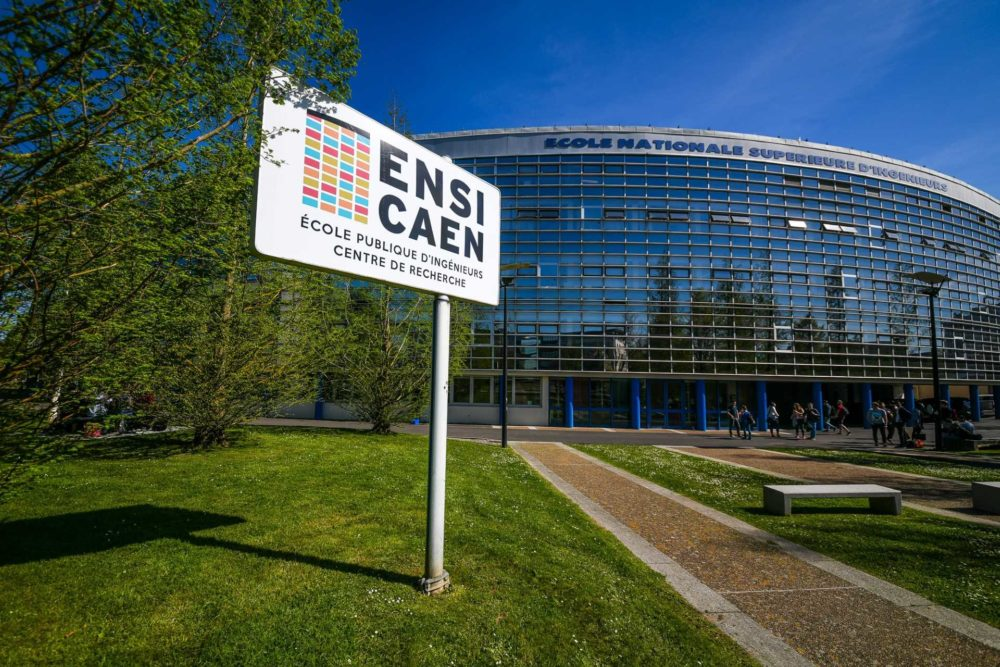
\includegraphics[scale=0.1]{figuras/ENSICAEN-batiment-A.jpg}
    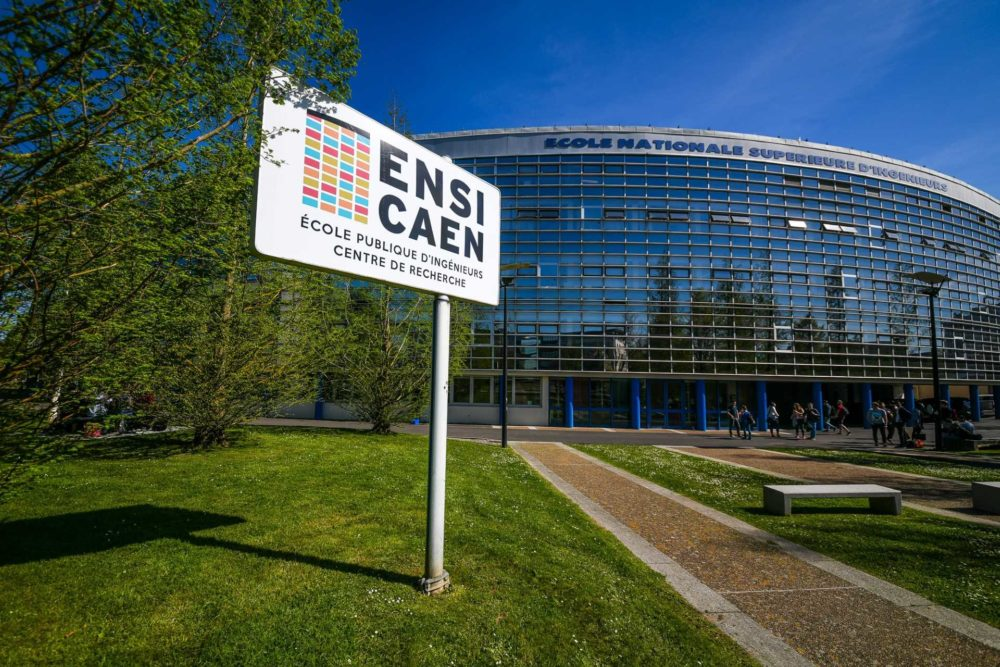
\includegraphics[scale=0.1]{figuras/ENSICAEN-batiment-A.jpg}
    %\caption{Caption}
    \label{fig:my_label}
\end{figure}
    
\end{frame}

\begin{frame}{Bootlin}

    \begin{itemize}
        \item Empresa prestadora de serviços e treinamentos em Linux embarcado
        \item Forte presença no mundo do software livre
        \item Escritórios em Toulouse, Lyon e Orange
    \end{itemize}
    
    \begin{figure}
        \centering
        
\includegraphics[scale=0.6]{figuras/bootlin_logo.png}
        %\caption{Logo da empresa}
        \label{fig:my_label}
    \end{figure}

\end{frame}
